\documentclass{article}\usepackage[]{graphicx}\usepackage[]{xcolor}
% maxwidth is the original width if it is less than linewidth
% otherwise use linewidth (to make sure the graphics do not exceed the margin)
\makeatletter
\def\maxwidth{ %
  \ifdim\Gin@nat@width>\linewidth
    \linewidth
  \else
    \Gin@nat@width
  \fi
}
\makeatother

\definecolor{fgcolor}{rgb}{0.345, 0.345, 0.345}
\newcommand{\hlnum}[1]{\textcolor[rgb]{0.686,0.059,0.569}{#1}}%
\newcommand{\hlsng}[1]{\textcolor[rgb]{0.192,0.494,0.8}{#1}}%
\newcommand{\hlcom}[1]{\textcolor[rgb]{0.678,0.584,0.686}{\textit{#1}}}%
\newcommand{\hlopt}[1]{\textcolor[rgb]{0,0,0}{#1}}%
\newcommand{\hldef}[1]{\textcolor[rgb]{0.345,0.345,0.345}{#1}}%
\newcommand{\hlkwa}[1]{\textcolor[rgb]{0.161,0.373,0.58}{\textbf{#1}}}%
\newcommand{\hlkwb}[1]{\textcolor[rgb]{0.69,0.353,0.396}{#1}}%
\newcommand{\hlkwc}[1]{\textcolor[rgb]{0.333,0.667,0.333}{#1}}%
\newcommand{\hlkwd}[1]{\textcolor[rgb]{0.737,0.353,0.396}{\textbf{#1}}}%
\let\hlipl\hlkwb

\usepackage{framed}
\makeatletter
\newenvironment{kframe}{%
 \def\at@end@of@kframe{}%
 \ifinner\ifhmode%
  \def\at@end@of@kframe{\end{minipage}}%
  \begin{minipage}{\columnwidth}%
 \fi\fi%
 \def\FrameCommand##1{\hskip\@totalleftmargin \hskip-\fboxsep
 \colorbox{shadecolor}{##1}\hskip-\fboxsep
     % There is no \\@totalrightmargin, so:
     \hskip-\linewidth \hskip-\@totalleftmargin \hskip\columnwidth}%
 \MakeFramed {\advance\hsize-\width
   \@totalleftmargin\z@ \linewidth\hsize
   \@setminipage}}%
 {\par\unskip\endMakeFramed%
 \at@end@of@kframe}
\makeatother

\definecolor{shadecolor}{rgb}{.97, .97, .97}
\definecolor{messagecolor}{rgb}{0, 0, 0}
\definecolor{warningcolor}{rgb}{1, 0, 1}
\definecolor{errorcolor}{rgb}{1, 0, 0}
\newenvironment{knitrout}{}{} % an empty environment to be redefined in TeX

\usepackage{alltt}
\usepackage[margin=1.0in]{geometry} % To set margins
\usepackage{amsmath}  % This allows me to use the align functionality.
                      % If you find yourself trying to replicate
                      % something you found online, ensure you're
                      % loading the necessary packages!
\usepackage{amsfonts} % Math font
\usepackage{fancyvrb}
\usepackage{hyperref} % For including hyperlinks
\usepackage[shortlabels]{enumitem}% For enumerated lists with labels specified
                                  % We had to run tlmgr_install("enumitem") in R
\usepackage{float}    % For telling R where to put a table/figure
\usepackage{natbib}        %For the bibliography
\bibliographystyle{apalike}%For the bibliography
\IfFileExists{upquote.sty}{\usepackage{upquote}}{}
\begin{document}


\begin{enumerate}
%%%%%%%%%%%%%%%%%%%%%%%%%%%%%%%%%%%%%%%%%%%%%%%%%%%%%%%%%%%%%%%%%%%%%%%%%%%%%%%%
%%%%%%%%%%%%%%%%%%%%%%%%%%%%%%%%%%%%%%%%%%%%%%%%%%%%%%%%%%%%%%%%%%%%%%%%%%%%%%%%
% Question 1
%%%%%%%%%%%%%%%%%%%%%%%%%%%%%%%%%%%%%%%%%%%%%%%%%%%%%%%%%%%%%%%%%%%%%%%%%%%%%%%%
%%%%%%%%%%%%%%%%%%%%%%%%%%%%%%%%%%%%%%%%%%%%%%%%%%%%%%%%%%%%%%%%%%%%%%%%%%%%%%%%
\item When conducting the work of Lab 11, we conducted the test that uses the
Central Limit Theorem even though the sample size was ``small" (i.e., $n<30$).
It turns out, that how ``far off" the $t$-test is can be computed using
a first-order Edgeworth approximation for the error. Below, we will do this 
for the the further observations.
\begin{enumerate}
  \item \cite{Boos00} note that 
  \begin{align*}
    P(T \leq t) \approx F_Z(t) + \underbrace{\frac{\text{skew}}{\sqrt{n}} \frac{(2t^2+1)}{6} f_Z(t)}_{\textrm{error}},
  \end{align*}
  where $f_Z(\cdot)$ and $F_Z(\cdot)$ are the Gaussian PDF and CDF and skew is the
  skewness of the data. What is the potential error in the computation of the 
  $p$-value when testing $H_0: \mu_X=0; H_a: \mu_X<0$ using the zebra finch further data? 
  
\begin{knitrout}
\definecolor{shadecolor}{rgb}{0.969, 0.969, 0.969}\color{fgcolor}\begin{kframe}
\begin{alltt}
\hlkwd{library}\hldef{(e1071)}
\hldef{finch_data} \hlkwb{=} \hlkwd{read_csv}\hldef{(}\hlsng{"zebrafinches.csv"}\hldef{)}
\hlcom{# View(finch_data)}
\hldef{further} \hlkwb{=} \hldef{finch_data}\hlopt{$}\hldef{further}
\hldef{n} \hlkwb{=} \hlkwd{length}\hldef{(further)}
\hldef{t} \hlkwb{=} \hlkwd{mean}\hldef{(further)} \hlopt{/} \hldef{(}\hlkwd{sd}\hldef{(further)}\hlopt{/}\hlkwd{sqrt}\hldef{(n))}

\hldef{error} \hlkwb{=} \hldef{(}\hlkwd{skewness}\hldef{(further)} \hlopt{/} \hlkwd{sqrt}\hldef{(n))} \hlopt{*} \hldef{((}\hlnum{2}\hlopt{*}\hldef{t}\hlopt{^}\hlnum{2} \hlopt{+} \hlnum{1}\hldef{)} \hlopt{/} \hlnum{6}\hldef{)} \hlopt{*} \hlkwd{dnorm}\hldef{(t)}
\hldef{error}
\end{alltt}
\begin{verbatim}
## [1] -1.226006e-13
\end{verbatim}
\end{kframe}
\end{knitrout}

  \item Compute the error for $t$ statistics from -10 to 10 and plot a line
  that shows the error across $t$. Continue to use the skewness and 
  the sample size for the zebra finch further data.
  
\begin{knitrout}
\definecolor{shadecolor}{rgb}{0.969, 0.969, 0.969}\color{fgcolor}\begin{kframe}
\begin{alltt}
\hlkwd{library}\hldef{(ggplot2)}
\hlkwd{library}\hldef{(e1071)}
\hldef{finch_data} \hlkwb{=} \hlkwd{read_csv}\hldef{(}\hlsng{"zebrafinches.csv"}\hldef{)}
\hldef{further} \hlkwb{=} \hldef{finch_data}\hlopt{$}\hldef{further}
\hldef{n} \hlkwb{=} \hlkwd{length}\hldef{(further)}
\hldef{t_vals} \hlkwb{=} \hlkwd{seq}\hldef{(}\hlopt{-}\hlnum{10}\hldef{,} \hlnum{10}\hldef{,} \hlkwc{by} \hldef{=} \hlnum{0.1}\hldef{)}
\hldef{error_vals} \hlkwb{=} \hldef{(}\hlkwd{skewness}\hldef{(further)} \hlopt{/} \hlkwd{sqrt}\hldef{(n))} \hlopt{*} \hldef{((}\hlnum{2}\hlopt{*}\hldef{t_vals}\hlopt{^}\hlnum{2} \hlopt{+} \hlnum{1}\hldef{)} \hlopt{/} \hlnum{6}\hldef{)} \hlopt{*} \hlkwd{dnorm}\hldef{(t_vals)}
\hlcom{# error_vals}
\hldef{df} \hlkwb{=} \hlkwd{data.frame}\hldef{(t_vals, error_vals)}

\hlkwd{ggplot}\hldef{(df,} \hlkwd{aes}\hldef{(}\hlkwc{x} \hldef{= t_vals,} \hlkwc{y} \hldef{= error_vals))} \hlopt{+}
  \hlkwd{geom_line}\hldef{(}\hlkwc{color} \hldef{=} \hlsng{"blue"}\hldef{)} \hlopt{+}
  \hlkwd{labs}\hldef{(}\hlkwc{title} \hldef{=} \hlsng{"Approximation Error vs. t"}\hldef{,}
       \hlkwc{x} \hldef{=} \hlsng{"t value"}\hldef{,}
       \hlkwc{y} \hldef{=} \hlsng{"Approximation Error"}\hldef{)} \hlopt{+}
  \hlkwd{theme_minimal}\hldef{()}
\end{alltt}
\end{kframe}
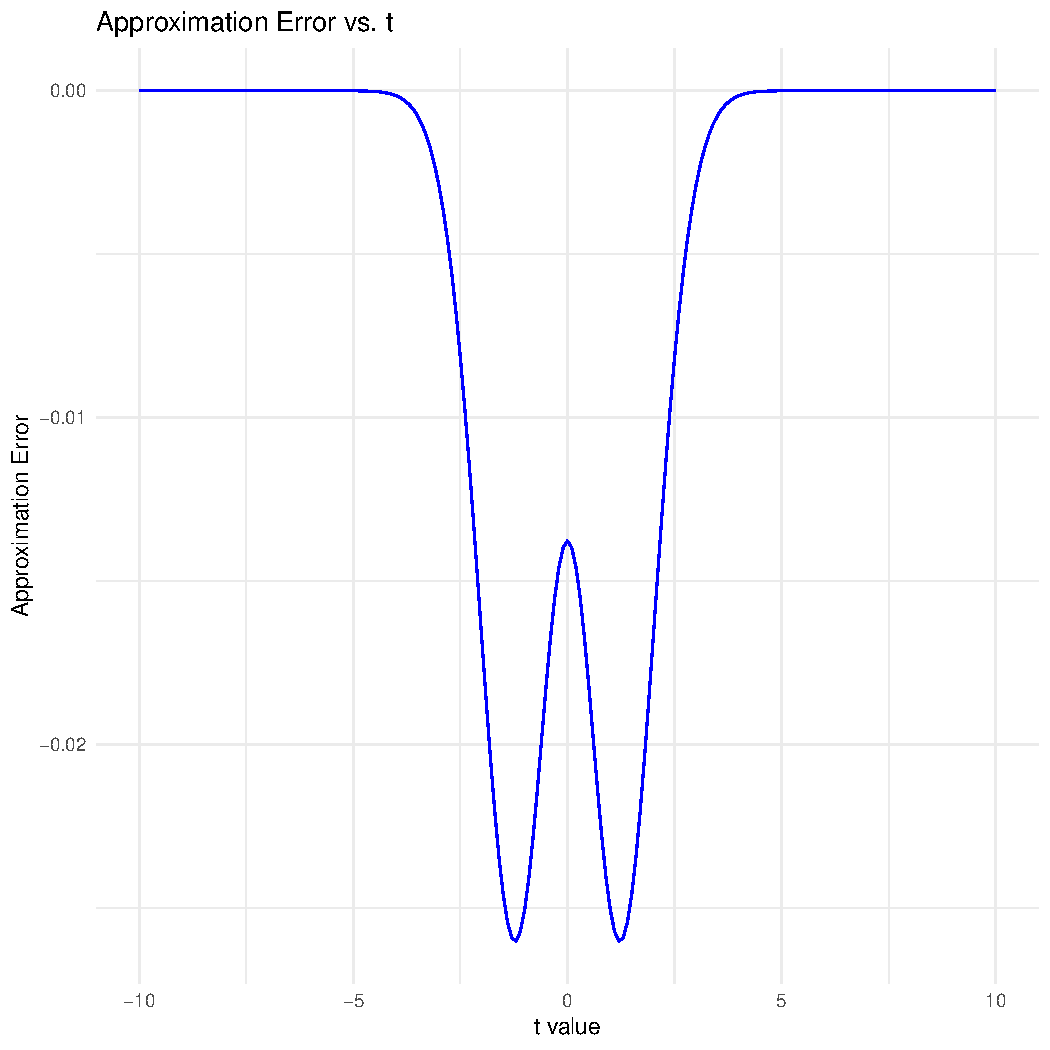
\includegraphics[width=\maxwidth]{figure/unnamed-chunk-3-1} 
\end{knitrout}

  \item Suppose we wanted to have a tail probability within 10\% of the desired
  $\alpha=0.05$. Recall we did a left-tailed test using the further data.
  How large of a sample size would we need? That is, we need
  to solve the error formula equal to 10\% of the desired left-tail probability:
  \[0.10 \alpha  \stackrel{set}{=} \underbrace{\frac{\text{skew}}{\sqrt{n}} \frac{(2t^2+1)}{6} f_Z(t)}_{\textrm{error}},\]
  which yields
  \[ n = \left(\frac{\text{skew}}{6(0.10\alpha)} (2t^2 + 1) f_Z(t)\right)^2.\]
\end{enumerate}

\begin{knitrout}
\definecolor{shadecolor}{rgb}{0.969, 0.969, 0.969}\color{fgcolor}\begin{kframe}
\begin{alltt}
\hlkwd{library}\hldef{(e1071)}

\hldef{finch_data} \hlkwb{=} \hlkwd{read_csv}\hldef{(}\hlsng{"zebrafinches.csv"}\hldef{)}
\hlcom{# View(finch_data)}
\hldef{further} \hlkwb{=} \hldef{finch_data}\hlopt{$}\hldef{further}
\hldef{alpha} \hlkwb{=} \hlnum{0.05}
\hldef{n} \hlkwb{=} \hlkwd{length}\hldef{(further)}
\hldef{t} \hlkwb{=} \hlkwd{qnorm}\hldef{(alpha)}
\hlkwd{skewness}\hldef{(further)}
\end{alltt}
\begin{verbatim}
## [1] -1.035507
\end{verbatim}
\begin{alltt}
\hldef{n} \hlkwb{=} \hldef{((}\hlkwd{skewness}\hldef{(further)}\hlopt{/}\hldef{(}\hlnum{6}\hlopt{*}\hlnum{0.1}\hlopt{*}\hlnum{0.05}\hldef{))} \hlopt{*} \hldef{(}\hlnum{2}\hlopt{*}\hldef{t}\hlopt{^}\hlnum{2} \hlopt{+} \hlnum{1}\hldef{)} \hlopt{*} \hlkwd{dnorm}\hldef{(t))}\hlopt{^}\hlnum{2}
\hldef{n}
\end{alltt}
\begin{verbatim}
## [1] 520.8876
\end{verbatim}
\end{kframe}
\end{knitrout}

%%%%%%%%%%%%%%%%%%%%%%%%%%%%%%%%%%%%%%%%%%%%%%%%%%%%%%%%%%%%%%%%%%%%%%%%%%%%%%%%
%%%%%%%%%%%%%%%%%%%%%%%%%%%%%%%%%%%%%%%%%%%%%%%%%%%%%%%%%%%%%%%%%%%%%%%%%%%%%%%%
% Question 3
%%%%%%%%%%%%%%%%%%%%%%%%%%%%%%%%%%%%%%%%%%%%%%%%%%%%%%%%%%%%%%%%%%%%%%%%%%%%%%%%
%%%%%%%%%%%%%%%%%%%%%%%%%%%%%%%%%%%%%%%%%%%%%%%%%%%%%%%%%%%%%%%%%%%%%%%%%%%%%%%%
\item Complete the following steps to revisit the analyses from lab 11 using the
bootstrap procedure.
\begin{enumerate}
\item Now, consider the zebra finch data. We do not know the generating distributions
for the closer, further, and difference data, so perform resampling to approximate the 
sampling distribution of the $T$ statistic:
  \[T = \frac{\bar{x}_r - 0}{s/\sqrt{n}},\]
  where $\bar{x}_r$ is the mean computed on the r$^{th}$ resample and $s$ is the
  sample standard deviation from the original samples. At the end, create an
  object called \texttt{resamples.null.closer}, for example, and store the 
  resamples shifted to ensure they are consistent with the null hypotheses at the average 
  (i.e., here ensure the shifted resamples are 0 on average, corresponding
  to $t=0$, for each case). 
  
\begin{knitrout}
\definecolor{shadecolor}{rgb}{0.969, 0.969, 0.969}\color{fgcolor}\begin{kframe}
\begin{alltt}
\hlkwd{library}\hldef{(e1071)}

\hldef{finch_data} \hlkwb{=} \hlkwd{read_csv}\hldef{(}\hlsng{"zebrafinches.csv"}\hldef{)}
\hldef{further} \hlkwb{=} \hldef{finch_data}\hlopt{$}\hldef{further}
\hldef{closer} \hlkwb{=} \hldef{finch_data}\hlopt{$}\hldef{closer}
\hldef{diff} \hlkwb{=} \hldef{finch_data}\hlopt{$}\hldef{diff}
\hldef{n} \hlkwb{=} \hlkwd{nrow}\hldef{(finch_data)}
\hldef{m0} \hlkwb{=} \hlnum{0}

\hlkwd{set.seed}\hldef{(}\hlnum{123}\hldef{)}
\hldef{R} \hlkwb{<-} \hlnum{10000}
\hldef{further_resamples} \hlkwb{<-} \hlkwd{tibble}\hldef{(}\hlkwc{t.stats}\hldef{=}\hlkwd{rep}\hldef{(}\hlnum{NA}\hldef{, R))}
\hldef{closer_resamples} \hlkwb{=} \hlkwd{tibble}\hldef{(}\hlkwc{t.stats}\hldef{=}\hlkwd{rep}\hldef{(}\hlnum{NA}\hldef{, R))}
\hldef{diff_resamples} \hlkwb{=} \hlkwd{tibble}\hldef{(}\hlkwc{t.stats}\hldef{=}\hlkwd{rep}\hldef{(}\hlnum{NA}\hldef{, R))}
\hlkwa{for}\hldef{(i} \hlkwa{in} \hlnum{1}\hlopt{:}\hldef{R)\{}
  \hldef{new_further_resample} \hlkwb{=} \hlkwd{sample}\hldef{(further,}
                     \hlkwc{size} \hldef{= n,}
                     \hlkwc{replace} \hldef{= T)}

  \hldef{new_closer_resample} \hlkwb{=} \hlkwd{sample}\hldef{(closer,}
                     \hlkwc{size} \hldef{= n,}
                     \hlkwc{replace} \hldef{= T)}

  \hldef{new_diff_resample} \hlkwb{=} \hlkwd{sample}\hldef{(diff,}
                     \hlkwc{size} \hldef{= n,}
                     \hlkwc{replace} \hldef{= T)}

\hldef{further_resamples}\hlopt{$}\hldef{t.stats[i]} \hlkwb{<-} \hlkwd{mean}\hldef{(new_further_resample)}\hlopt{/}\hldef{(}\hlkwd{sd}\hldef{(further)}\hlopt{/}\hlkwd{sqrt}\hldef{(n))}
\hldef{closer_resamples}\hlopt{$}\hldef{t.stats[i]} \hlkwb{=} \hlkwd{mean}\hldef{(new_closer_resample)}\hlopt{/}\hldef{(}\hlkwd{sd}\hldef{(closer)}\hlopt{/}\hlkwd{sqrt}\hldef{(n))}
\hldef{diff_resamples}\hlopt{$}\hldef{t.stats[i]} \hlkwb{=} \hlkwd{mean}\hldef{(new_diff_resample)}\hlopt{/}\hldef{(}\hlkwd{sd}\hldef{(diff)}\hlopt{/}\hlkwd{sqrt}\hldef{(n))}
\hldef{\}}
\hlcom{# View(further_resamples)}

\hldef{resamples.null.farther} \hlkwb{=} \hldef{further_resamples}\hlopt{$}\hldef{t.stats} \hlopt{-} \hlkwd{mean}\hldef{(further_resamples}\hlopt{$}\hldef{t.stats)}
\hldef{resamples.null.closer} \hlkwb{=} \hldef{closer_resamples}\hlopt{$}\hldef{t.stats} \hlopt{-} \hlkwd{mean}\hldef{(closer_resamples}\hlopt{$}\hldef{t.stats)}
\hldef{resamples.null.diff} \hlkwb{=} \hldef{diff_resamples}\hlopt{$}\hldef{t.stats} \hlopt{-} \hlkwd{mean}\hldef{(diff_resamples}\hlopt{$}\hldef{t.stats)}
\end{alltt}
\end{kframe}
\end{knitrout}
  
  \item Compute the bootstrap $p$-value for each test using the shifted resamples. 
  How do these compare to the $t$-test $p$-values?
  
\begin{knitrout}
\definecolor{shadecolor}{rgb}{0.969, 0.969, 0.969}\color{fgcolor}\begin{kframe}
\begin{verbatim}
## [1] 0
## [1] 0
## [1] 0
\end{verbatim}
\end{kframe}
\end{knitrout}
    \item What is the 5$^{th}$ percentile of the shifted resamples under the null hypothesis? 
  Note this value approximates $t_{0.05, n-1}$. Compare these values in each case.
  
\begin{knitrout}
\definecolor{shadecolor}{rgb}{0.969, 0.969, 0.969}\color{fgcolor}\begin{kframe}
\begin{verbatim}
## [1] "-1.68480212921038 is the 5th percentile of the shifted further data resamples"
## [1] "-1.59314617071328 is the 5th percentile of the shifted closer data resamples"
## [1] "-1.56409157711738 is the 5th percentile of the shifted diff data resamples"
\end{verbatim}
\end{kframe}
\end{knitrout}
  
  \item Compute the bootstrap confidence intervals using the resamples. How do these 
  compare to the $t$-test confidence intervals?
  
\begin{knitrout}
\definecolor{shadecolor}{rgb}{0.969, 0.969, 0.969}\color{fgcolor}\begin{kframe}
\begin{alltt}
\hlkwd{library}\hldef{(e1071)}

\hldef{finch_data} \hlkwb{=} \hlkwd{read_csv}\hldef{(}\hlsng{"zebrafinches.csv"}\hldef{)}
\hldef{further} \hlkwb{=} \hldef{finch_data}\hlopt{$}\hldef{further}
\hldef{closer} \hlkwb{=} \hldef{finch_data}\hlopt{$}\hldef{closer}
\hldef{diff} \hlkwb{=} \hldef{finch_data}\hlopt{$}\hldef{diff}
\hldef{n} \hlkwb{=} \hlkwd{nrow}\hldef{(finch_data)}
\hldef{m0} \hlkwb{=} \hlnum{0}

\hlkwd{set.seed}\hldef{(}\hlnum{123}\hldef{)}
\hldef{R} \hlkwb{<-} \hlnum{10000}
\hldef{further_resamples} \hlkwb{<-} \hlkwd{tibble}\hldef{(}\hlkwc{t.stats}\hldef{=}\hlkwd{rep}\hldef{(}\hlnum{NA}\hldef{, R))}
\hldef{closer_resamples} \hlkwb{=} \hlkwd{tibble}\hldef{(}\hlkwc{t.stats}\hldef{=}\hlkwd{rep}\hldef{(}\hlnum{NA}\hldef{, R))}
\hldef{diff_resamples} \hlkwb{=} \hlkwd{tibble}\hldef{(}\hlkwc{t.stats}\hldef{=}\hlkwd{rep}\hldef{(}\hlnum{NA}\hldef{, R))}
\hlkwa{for}\hldef{(i} \hlkwa{in} \hlnum{1}\hlopt{:}\hldef{R)\{}
  \hldef{new_further_resample} \hlkwb{=} \hlkwd{sample}\hldef{(further,}
                     \hlkwc{size} \hldef{= n,}
                     \hlkwc{replace} \hldef{= T)}

  \hldef{new_closer_resample} \hlkwb{=} \hlkwd{sample}\hldef{(closer,}
                     \hlkwc{size} \hldef{= n,}
                     \hlkwc{replace} \hldef{= T)}

  \hldef{new_diff_resample} \hlkwb{=} \hlkwd{sample}\hldef{(diff,}
                     \hlkwc{size} \hldef{= n,}
                     \hlkwc{replace} \hldef{= T)}

\hldef{further_resamples}\hlopt{$}\hldef{t.stats[i]} \hlkwb{<-} \hlkwd{mean}\hldef{(new_further_resample)}\hlopt{/}\hldef{(}\hlkwd{sd}\hldef{(further)}\hlopt{/}\hlkwd{sqrt}\hldef{(n))}
\hldef{closer_resamples}\hlopt{$}\hldef{t.stats[i]} \hlkwb{=} \hlkwd{mean}\hldef{(new_closer_resample)}\hlopt{/}\hldef{(}\hlkwd{sd}\hldef{(closer)}\hlopt{/}\hlkwd{sqrt}\hldef{(n))}
\hldef{diff_resamples}\hlopt{$}\hldef{t.stats[i]} \hlkwb{=} \hlkwd{mean}\hldef{(new_diff_resample)}\hlopt{/}\hldef{(}\hlkwd{sd}\hldef{(diff)}\hlopt{/}\hlkwd{sqrt}\hldef{(n))}
\hldef{\}}
\hlcom{# View(further_resamples)}

\hldef{resamples.null.further} \hlkwb{=} \hldef{further_resamples}\hlopt{$}\hldef{t.stats} \hlopt{-} \hlkwd{mean}\hldef{(further_resamples}\hlopt{$}\hldef{t.stats)}
\hldef{resamples.null.closer} \hlkwb{=} \hldef{closer_resamples}\hlopt{$}\hldef{t.stats} \hlopt{-} \hlkwd{mean}\hldef{(closer_resamples}\hlopt{$}\hldef{t.stats)}
\hldef{resamples.null.diff} \hlkwb{=} \hldef{diff_resamples}\hlopt{$}\hldef{t.stats} \hlopt{-} \hlkwd{mean}\hldef{(diff_resamples}\hlopt{$}\hldef{t.stats)}

\hldef{CI_further} \hlkwb{=} \hlkwd{quantile}\hldef{(resamples.null.further,} \hlkwd{c}\hldef{(}\hlnum{0.025}\hldef{,} \hlnum{0.975}\hldef{))}
\hldef{CI_closer} \hlkwb{=} \hlkwd{quantile}\hldef{(resamples.null.closer,} \hlkwd{c}\hldef{(}\hlnum{0.025}\hldef{,} \hlnum{0.975}\hldef{))}
\hldef{CI_diff} \hlkwb{=} \hlkwd{quantile}\hldef{(resamples.null.diff,} \hlkwd{c}\hldef{(}\hlnum{0.025}\hldef{,} \hlnum{0.975}\hldef{))}

\hldef{CI_further_t} \hlkwb{=} \hlkwd{mean}\hldef{(further)} \hlopt{+} \hlkwd{c}\hldef{(}\hlopt{-}\hlnum{1}\hldef{,} \hlnum{1}\hldef{)} \hlopt{*} \hlkwd{qt}\hldef{(}\hlnum{0.975}\hldef{,} \hlkwc{df} \hldef{= n}\hlopt{-}\hlnum{1}\hldef{)} \hlopt{*} \hlkwd{sd}\hldef{(further)}\hlopt{/}\hlkwd{sqrt}\hldef{(n)}
\hldef{CI_closer_t} \hlkwb{=} \hlkwd{mean}\hldef{(closer)} \hlopt{+} \hlkwd{c}\hldef{(}\hlopt{-}\hlnum{1}\hldef{,} \hlnum{1}\hldef{)} \hlopt{*} \hlkwd{qt}\hldef{(}\hlnum{0.975}\hldef{,} \hlkwc{df} \hldef{= n}\hlopt{-}\hlnum{1}\hldef{)} \hlopt{*} \hlkwd{sd}\hldef{(closer)}\hlopt{/}\hlkwd{sqrt}\hldef{(n)}
\hldef{CI_diff_t} \hlkwb{=} \hlkwd{mean}\hldef{(diff)} \hlopt{+} \hlkwd{c}\hldef{(}\hlopt{-}\hlnum{1}\hldef{,} \hlnum{1}\hldef{)} \hlopt{*} \hlkwd{qt}\hldef{(}\hlnum{0.975}\hldef{,} \hlkwc{df} \hldef{= n}\hlopt{-}\hlnum{1}\hldef{)} \hlopt{*} \hlkwd{sd}\hldef{(diff)}\hlopt{/}\hlkwd{sqrt}\hldef{(n)}
\hlcom{#Should I use resamples.null.data or just the data}
\hldef{CI_further}
\end{alltt}
\begin{verbatim}
##      2.5%     97.5% 
## -2.033830  1.826771
\end{verbatim}
\begin{alltt}
\hldef{CI_further_t}
\end{alltt}
\begin{verbatim}
## [1] -0.2565176 -0.1489313
\end{verbatim}
\begin{alltt}
\hldef{CI_closer}
\end{alltt}
\begin{verbatim}
##      2.5%     97.5% 
## -1.878078  1.926030
\end{verbatim}
\begin{alltt}
\hldef{CI_closer_t}
\end{alltt}
\begin{verbatim}
## [1] 0.1173875 0.1950586
\end{verbatim}
\begin{alltt}
\hldef{CI_diff}
\end{alltt}
\begin{verbatim}
##      2.5%     97.5% 
## -1.857155  2.032365
\end{verbatim}
\begin{alltt}
\hldef{CI_diff_t}
\end{alltt}
\begin{verbatim}
## [1] 0.2719028 0.4459921
\end{verbatim}
\end{kframe}
\end{knitrout}
  
\end{enumerate}
%%%%%%%%%%%%%%%%%%%%%%%%%%%%%%%%%%%%%%%%%%%%%%%%%%%%%%%%%%%%%%%%%%%%%%%%%%%%%%%%
%%%%%%%%%%%%%%%%%%%%%%%%%%%%%%%%%%%%%%%%%%%%%%%%%%%%%%%%%%%%%%%%%%%%%%%%%%%%%%%%
% Question 4
%%%%%%%%%%%%%%%%%%%%%%%%%%%%%%%%%%%%%%%%%%%%%%%%%%%%%%%%%%%%%%%%%%%%%%%%%%%%%%%%
%%%%%%%%%%%%%%%%%%%%%%%%%%%%%%%%%%%%%%%%%%%%%%%%%%%%%%%%%%%%%%%%%%%%%%%%%%%%%%%%
\item Complete the following steps to revisit the analyses from lab 11 using the
randomization procedure.
\begin{enumerate}
\item Now, consider the zebra finch data. We do not know the generating distributions
for the closer, further, and difference data, so perform the randomization procedure

\begin{knitrout}
\definecolor{shadecolor}{rgb}{0.969, 0.969, 0.969}\color{fgcolor}\begin{kframe}
\begin{alltt}
\hldef{randomization_test} \hlkwb{=} \hlkwa{function}\hldef{(}\hlkwc{data}\hldef{,} \hlkwc{mu0} \hldef{=} \hlnum{0}\hldef{,} \hlkwc{R} \hldef{=} \hlnum{10000}\hldef{)\{}
  \hldef{x_shift} \hlkwb{=} \hldef{data}\hlopt{-}\hldef{m0}
  \hldef{rand} \hlkwb{=} \hlkwd{tibble}\hldef{(}\hlkwc{xbars} \hldef{=} \hlkwd{rep}\hldef{(}\hlnum{NA}\hldef{, R))}

  \hlkwa{for} \hldef{(i} \hlkwa{in} \hlnum{1}\hlopt{:}\hldef{R)\{}
    \hldef{curr.rand} \hlkwb{=} \hldef{x_shift} \hlopt{*} \hlkwd{sample}\hldef{(}\hlkwd{c}\hldef{(}\hlopt{-}\hlnum{1}\hldef{,}\hlnum{1}\hldef{),}
                          \hlkwd{length}\hldef{(x_shift),}
                          \hlkwc{replace} \hldef{= T)}
    \hldef{rand}\hlopt{$}\hldef{xbars[i]} \hlkwb{=} \hlkwd{mean}\hldef{(curr.rand)}
  \hldef{\}}

  \hldef{rand} \hlkwb{=} \hldef{rand |>}
    \hlkwd{mutate}\hldef{(}
      \hlkwc{xbars} \hldef{= xbars} \hlopt{+} \hldef{mu0}
    \hldef{)}
  \hlkwd{return}\hldef{(rand}\hlopt{$}\hldef{xbars)}
\hldef{\}}

\hldef{finch_data} \hlkwb{=} \hlkwd{read_csv}\hldef{(}\hlsng{"zebrafinches.csv"}\hldef{)}

\hldef{rand_further} \hlkwb{=} \hlkwd{randomization_test}\hldef{(finch_data}\hlopt{$}\hldef{further)}
\hldef{rand_closer} \hlkwb{=} \hlkwd{randomization_test}\hldef{(finch_data}\hlopt{$}\hldef{closer)}
\hldef{rand_diff} \hlkwb{=} \hlkwd{randomization_test}\hldef{(finch_data}\hlopt{$}\hldef{diff)}
\end{alltt}
\end{kframe}
\end{knitrout}

  \item Compute the randomization test $p$-value for each test.
  
\begin{knitrout}
\definecolor{shadecolor}{rgb}{0.969, 0.969, 0.969}\color{fgcolor}\begin{kframe}
\begin{alltt}
\hldef{randomization_test} \hlkwb{=} \hlkwa{function}\hldef{(}\hlkwc{data}\hldef{,} \hlkwc{mu0} \hldef{=} \hlnum{0}\hldef{,} \hlkwc{R} \hldef{=} \hlnum{10000}\hldef{)\{}
  \hldef{x_shift} \hlkwb{=} \hldef{data}\hlopt{-}\hldef{m0}
  \hldef{rand} \hlkwb{=} \hlkwd{tibble}\hldef{(}\hlkwc{xbars} \hldef{=} \hlkwd{rep}\hldef{(}\hlnum{NA}\hldef{, R))}

  \hlkwa{for} \hldef{(i} \hlkwa{in} \hlnum{1}\hlopt{:}\hldef{R)\{}
    \hldef{curr.rand} \hlkwb{=} \hldef{x_shift} \hlopt{*} \hlkwd{sample}\hldef{(}\hlkwd{c}\hldef{(}\hlopt{-}\hlnum{1}\hldef{,}\hlnum{1}\hldef{),}
                          \hlkwd{length}\hldef{(x_shift),}
                          \hlkwc{replace} \hldef{= T)}
    \hldef{rand}\hlopt{$}\hldef{xbars[i]} \hlkwb{=} \hlkwd{mean}\hldef{(curr.rand)}
  \hldef{\}}

  \hldef{rand} \hlkwb{=} \hldef{rand |>}
    \hlkwd{mutate}\hldef{(}
      \hlkwc{xbars} \hldef{= xbars} \hlopt{+} \hldef{mu0}
    \hldef{)}
  \hlkwd{return}\hldef{(rand}\hlopt{$}\hldef{xbars)}
\hldef{\}}

\hldef{finch_data} \hlkwb{=} \hlkwd{read_csv}\hldef{(}\hlsng{"zebrafinches.csv"}\hldef{)}

\hldef{rand_further} \hlkwb{=} \hlkwd{randomization_test}\hldef{(finch_data}\hlopt{$}\hldef{further)}
\hldef{rand_closer} \hlkwb{=} \hlkwd{randomization_test}\hldef{(finch_data}\hlopt{$}\hldef{closer)}
\hldef{rand_diff} \hlkwb{=} \hlkwd{randomization_test}\hldef{(finch_data}\hlopt{$}\hldef{diff)}

\hldef{pval_randomization} \hlkwb{=} \hlkwa{function}\hldef{(}\hlkwc{data}\hldef{,} \hlkwc{rand_samples}\hldef{,} \hlkwc{mu0} \hldef{=} \hlnum{0}\hldef{)\{}
  \hldef{delta} \hlkwb{=} \hlkwd{abs}\hldef{(}\hlkwd{mean}\hldef{(data)} \hlopt{-} \hldef{mu0)}
  \hldef{low} \hlkwb{=} \hldef{mu0} \hlopt{-} \hldef{delta}
  \hldef{high} \hlkwb{=} \hldef{mu0} \hlopt{-} \hldef{delta}
  \hlkwd{mean}\hldef{(rand_samples} \hlopt{<=} \hldef{low)} \hlopt{+} \hlkwd{mean}\hldef{(rand_samples} \hlopt{>=} \hldef{high)}
\hldef{\}}

\hldef{pval_further} \hlkwb{=} \hlkwd{pval_randomization}\hldef{(finch_data}\hlopt{$}\hldef{further, rand_further)}
\hldef{pval_closer} \hlkwb{=} \hlkwd{pval_randomization}\hldef{(finch_data}\hlopt{$}\hldef{closer, rand_closer)}
\hldef{pval_diff} \hlkwb{=} \hlkwd{pval_randomization}\hldef{(finch_data}\hlopt{$}\hldef{diff, rand_diff)}

\hldef{pval_further}
\end{alltt}
\begin{verbatim}
## [1] 1
\end{verbatim}
\begin{alltt}
\hldef{pval_closer}
\end{alltt}
\begin{verbatim}
## [1] 1
\end{verbatim}
\begin{alltt}
\hldef{pval_diff}
\end{alltt}
\begin{verbatim}
## [1] 1
\end{verbatim}
\end{kframe}
\end{knitrout}
  
  \item Compute the randomization confidence interval by iterating over values of $\mu_0$.\\
  \textbf{Hint:} You can ``search" for the lower bound from $Q_1$ and subtracting by 0.0001, 
  and the upper bound using $Q_3$ and increasing by 0.0001. You will continue until you find 
  the first value for which the two-sided $p$-value is greater than or equal to 0.05.
\end{enumerate}
%%%%%%%%%%%%%%%%%%%%%%%%%%%%%%%%%%%%%%%%%%%%%%%%%%%%%%%%%%%%%%%%%%%%%%%%%%%%%%%%
%%%%%%%%%%%%%%%%%%%%%%%%%%%%%%%%%%%%%%%%%%%%%%%%%%%%%%%%%%%%%%%%%%%%%%%%%%%%%%%%
% Optional Question
%%%%%%%%%%%%%%%%%%%%%%%%%%%%%%%%%%%%%%%%%%%%%%%%%%%%%%%%%%%%%%%%%%%%%%%%%%%%%%%%
%%%%%%%%%%%%%%%%%%%%%%%%%%%%%%%%%%%%%%%%%%%%%%%%%%%%%%%%%%%%%%%%%%%%%%%%%%%%%%%%
\item \textbf{Optional Challenge:} In this lab, you performed resampling to 
approximate the sampling distribution of the $T$ statistic using
\[T = \frac{\bar{x}_r - 0}{s/\sqrt{n}}.\]
I'm curious whether it is better/worse/similar if we computed the statistics
using the sample standard deviation of the resamples ($s_r$), instead of the 
original sample ($s$)
  \[T = \frac{\bar{x}_r - 0}{s_r/\sqrt{n}}.\]
\begin{enumerate}
  \item Perform a simulation study to evaluate the Type I error for conducting this
hypothesis test both ways.
  \item Using the same test case(s) as part (a), compute bootstrap confidence 
  intervals and assess their coverage -- how often do we `capture' the parameter
of interest?
\end{enumerate}
%%%%%%%%%%%%%%%%%%%%%%%%%%%%%%%%%%%%%%%%%%%%%%%%%%%%%%%%%%%%%%%%%%%%%%%%%%%%%%%%
%%%%%%%%%%%%%%%%%%%%%%%%%%%%%%%%%%%%%%%%%%%%%%%%%%%%%%%%%%%%%%%%%%%%%%%%%%%%%%%%
% End Document
%%%%%%%%%%%%%%%%%%%%%%%%%%%%%%%%%%%%%%%%%%%%%%%%%%%%%%%%%%%%%%%%%%%%%%%%%%%%%%%%
%%%%%%%%%%%%%%%%%%%%%%%%%%%%%%%%%%%%%%%%%%%%%%%%%%%%%%%%%%%%%%%%%%%%%%%%%%%%%%%%
\end{enumerate}
\bibliography{bibliography}
\end{document}

